% arara: xelatex: {synctex: true}
% arara: indent: {overwrite: yes}
\documentclass[]{IMTexam}

\usepackage[enums]{IMTtikz}

\givecredits
\author{Isabella B.}
\USPN{11810773}
\date{}
\lecture{Física I} % disciplina
\lcode{4302111}
\hwtype{Resolução} % o que é
\examname{Provinha VI} % prova

\begin{document}

\maketitle

Foguetes podem ser considerados como sistemas de massa variável. Suponhamos que o nosso objetivo seja construir um foguete que voe o mais alto possível. Qual é a melhor maneira de atingir esse objetivo? Seria gastar todo o combustível no começo, soltarmos aos poucos, ou talvez um meio termo? Analisaremos este problema nesta provinha.

\begin{questions}

	\question \label{ques:q1}
	Faremos primeiro o caso em que desprezamos a força da gravidade.

	\begin{figure}[H]
		\centering
		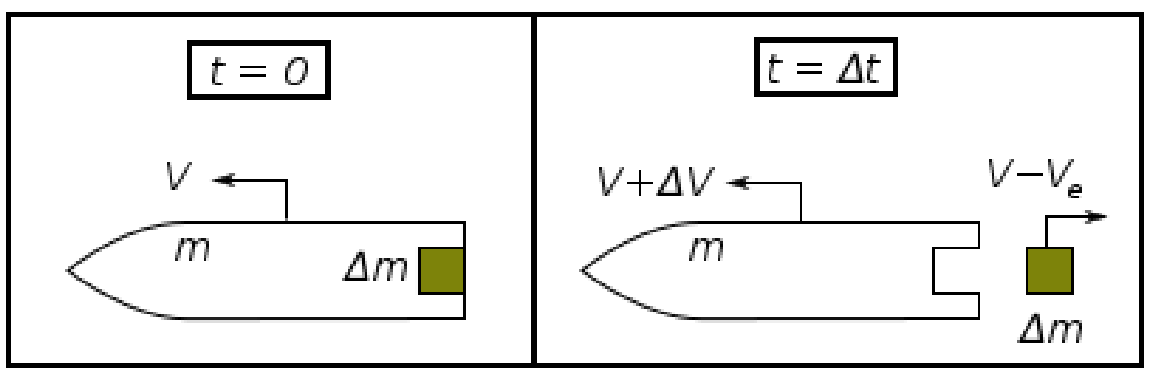
\includegraphics[width=0.7\linewidth]{screenshot001}
		\caption{Ejeção de um pacote de combustível de massa $ \Delta m $.}
		\label{fig:fig1}
	\end{figure}

	Veja a Figura \ref{fig:fig1}. Suponha que, em um intervalo de tempo $ \Delta t $, uma massa $ \Delta m $ de combustível é ejetada com velocidade ve em relação ao foguete. Orientamos o eixo positivo do deslocamento do foguete para a esquerda na figura acima, de forma que $ v > 0 $.
	\begin{parts}
		\part \label{part:q1a} Como não há forças externas do problema, use a conservação do momento linear total para achar a diferença de velocidade $ \Delta v $ que o foguete ganha em termos de $ m, \Delta m $ e $ v_e $.

		\begin{solution}

		\end{solution}

		\part \label{part:q1b} Divida o resultado acima por $ \Delta t $ e tome o limite $ \Delta t \to  0 $. Se definirmos a massa restante no foguete $ m(t) $ de sorte que $ m(0) = m + \Delta m $ e $ m(\Delta t) = m $, mostre que atua no foguete uma força de propulsão $ F_p = -v_e\,\dot{m} $.

		\begin{solution}

		\end{solution}

		\part \label{part:q1c} Dado que a massa inicial do foguete é $ m_0 $ e a final, $ m_f < m_0 $, resolva a equação diferencial encontrada no item anterior e prove que a diferença de velocidade entre os instantes final e inicial é dada por
		\begin{equation}\label{eq:DeltaV}
			\Delta v=v_e\ln\del{\dfrac{m_0}{m_f}}
		\end{equation}

		\begin{solution}

		\end{solution}
	\end{parts}

	\question \label{ques:q2}
	Agora introduziremos gravidade no problema. Inicialmente, temos um foguete parado na superfície da Terra apontado diretamente para cima.
	\begin{parts}
		\part \label{part:q2a} Escreva a segunda lei de Newton para o foguete, considerando aceleração da gravidade $ g $ constante.

		\begin{solution}

		\end{solution}

		\part \label{part:q2b} Isole a aceleração $ a=\dot{v}=\ddot{h} $ da segunda lei de Newton e mostre que
		\begin{equation}\label{eq:aoft}
			a(t)=-g-v_e\,\dod{}{t}\ln\del{m(t)}
		\end{equation}

		\begin{solution}

		\end{solution}

		\part \label{part:q2c} Suponhamos que o foguete saia do chão com velocidade nula e que sua massa inicial total seja $ m_0 $, contando com o combustível. A partir da equação \ref{eq:aoft}, encontre o fluxo inicial de massa $ \envert{\dot{m}(0)}=-\dot{m}(0) $ mínimo para que o foguete saia do chão, em termos de $ m_0, g $ e $ v_e $.

		\begin{solution}

		\end{solution}

		\part \label{part:q2d} Usando a equação \ref{eq:aoft}, prove que a velocidade $ v(t) $ é dada por:
		\[ v(t)=-g\,t-v_e\ln\del{\dfrac{m(t)}{m_0}} \]

		\begin{solution}

		\end{solution}

		\part \label{part:q2e} Suponhamos que o foguete saia do chão, $ h(0) = 0 $, e que demore um tempo $ t_I $ para consumir todo o combustível, de forma que ele atinja uma altura intermediária $ h(t_I)=H_I $ e que a massa do foguete sem combustível seja $ m(t_I) = m_f $. Nestas condições, integre a equação da velocidade $ v(t) $ encontrada acima para encontrar a seguinte relação para $ H_I $:
		\[ H_I=-\dfrac{1}{2}g\,t_I^{2}-v_e\int_{0}^{t_I}\ln\del{\dfrac{m(t)}{m_0}}\dif t. \]

		\begin{solution}

		\end{solution}

		\part \label{part:q2f} Se, após o combustível ter acabado, o foguete tiver uma velocidade $ v_I = v(t_I) $ positiva, então ele ainda subirá mais um pouco. Sabendo que só a força peso atua no foguete para $ t > t_I $, prove que sua altura máxima será
		\begin{align}
			H & =H_I+\dfrac{v_I^{2}}{2g}\nonumber                                                                   \\
			  & =\dfrac{\del{\Delta v}^{2}}{2g}-v_e\int_{0}^{t_I}\ln\del{\dfrac{m(t)}{m_f}}\dif t,\label{eq:maxH}
		\end{align}
		onde $ \Delta v $ está definido em \ref{eq:DeltaV}.

		\begin{solution}

		\end{solution}
	\end{parts}

	\question \label{ques:q3}
	A expressão para a altura máxima encontrada na equação \ref{eq:maxH} é genérica, e depende de como a massa do foguete (com combustível) $ m(t) $ diminui com o tempo. Para os itens a seguir, vamos assumir um modelo simples em que a massa do foguete é dada por $ m(t) = m0e-\alpha t $, para $ t \geqslant 0 $ e $ a $ uma constante positiva.
	\begin{parts}
		\part \label{part:q3a} Encontre o tempo $ t_I $ quando o combustível do foguete acaba em termos de $ \alpha , m_f $ e $ m_0 $.

		\begin{solution}

		\end{solution}

		\part \label{part:q3b} Usando o que foi encontrado no item \ref{ques:q2}.\ref{part:q2c}, mostre que $ \alpha $ deve ser maior que $ g/v_e $ para que o foguete não só saia do chão, mas para que continue acelerando enquanto houver combustível.

		\begin{solution}

		\end{solution}

		\part \label{part:q3c} Prove que a altura máxima do foguete neste caso é dada por
		\[ H=\dfrac{v_e^{2}}{2g}\sbr{\ln\del{\dfrac{m_0}{m_f}}}^{2}\del{1-\dfrac{g}{\alpha\,v_e}} \]

		\begin{solution}

		\end{solution}

		\part \label{part:q3d} Esboce o gráfico de $ H(\alpha) $ como função do parâmetro $ \alpha $, para $ \alpha > g/v_e $, e prove que $ H(\alpha) $ não possui valor máximo, mas que, para todo $ \alpha > 0 $,
		\begin{equation}\label{key}
			H(\alpha)<H_{\text{máx}}=\lim\limits_{\alpha\to\infty}H(\alpha)=\dfrac{v_e^{2}}{2g}\sbr{\ln\del{\dfrac{m_0}{m_f}}}^{2}
		\end{equation}

		\begin{solution}

		\end{solution}

		\part \label{part:q3e} O foguete voa mais alto se gastar o combustível lenta ou rapidamente? Por quê? Com base em \ref{eq:maxH}, argumente por que sua resposta vale no caso de uma função $ m(t) $ genérica --- não necessariamente exponencial --- mantidos constantes $ m_0, m_f, v_e $ e $ g $?

		\begin{solution}

		\end{solution}
	\end{parts}

	\extra{Questões extra}

	\question \label{ques:q4}
	A análise feita na questão 3 nos leva a crer que maximizamos a altura máxima atingida pelo foguete se tomarmos o limite $ \alpha  \to  +\infty $. Essa situação corresponderia a gastarmos todo o combustível instantaneamente em $ t = 0 $, assim que sairmos do chão. Contudo, temos de ser muito cuidadosos com a matemática subjacente:
	\begin{parts}
		\part \label{part:q4a} Antes do lançamento, o foguete está parado no chão, portanto $ m(t) = m_0 $ para $ t < 0 $. Dito isso, mostre que $\lim\limits_{\alpha \to \infty} m(t) = m_0\del{1 - \theta (t)} $, onde $ \theta (t) $ é a função degrau, definida por
		\[ \theta(t)=\begin{cases}
				1, & \text{se }t\geqslant0 \\
				0, & \text{se }t<0
			\end{cases} \]
		Faça um esboço de $ \lim\limits_{\alpha \to \infty} m(t) $.

		\begin{solution}

		\end{solution}

		\part \label{part:q4b} Prove que o fluxo de massa $ \envert{\dot{m}(t)}=-\dot{m}(t) $ no limite $ \alpha\to \infty $ é zero para $ t\neq0 $ e que não está definido em $ t = 0 $. Portanto, $\lim\limits_{\alpha\to +\infty}\envert{\dot{m}(t)}$ \textbf{não} está bem definida como função em $\mathbb{R}$.

		\begin{solution}

		\end{solution}

		\part \label{part:q4c} Apesar disso, ainda podemos realizar algumas operações em $\lim\limits_{\alpha\to +\infty}\envert{\dot{m}(t)}$ que normalmente se fariam com funções bem definidas. Em particular, podemos integrá-la, já que sua ``primitiva'' --- $\lim\limits_{\alpha\to +\infty}m(t)$ está bem definida para $ t\in\mathbb{R} $. Definimos a ``função'' delta de Dirac\footnote{Como estávamos argumentando, função não é o nome apropriado para $ \delta (t) $. De fato, a extensão matematicamente rigorosa mais próxima do que queremos dizer são as distribuições, que são uma generalização de funções.} por $ \delta (t) = \lim\limits_{\alpha \to +\infty}\envert{\dot{m}(t)}/m_0 $. Mostre que
		\[ \int_{I}\delta(t) \dif t = 1, \]
		para qualquer intervalo aberto $ I\subseteq\mathbb{R} $ que contenha $ 0 $.

		\begin{solution}

		\end{solution}
	\end{parts}

	\question \label{ques:q5}
	Poderíamos ter pensado da seguinte forma ao resolver o problema da questão \ref{ques:q2}: calculamos a variação da energia mecânica $ \Delta E_M $ entre os instantes inicial e final --- quando o foguete atinge sua altura máxima $ H $ --- e o trabalho $ W_p $ realizado pela força de propulsão $ F_p = -v_e\,\dot{m} $ neste percurso. Assim, acharíamos a altura máxima $ H $ através da relação $ \Delta E_M = W_p $.

	Mostre que, em geral, $ \Delta E_M \neq W_p $ para o modelo da questão \ref{ques:q3} e dê uma explicação para este aparente paradoxo.

\end{questions}
\end{document}
